242. \begin{figure}[ht!]
\center{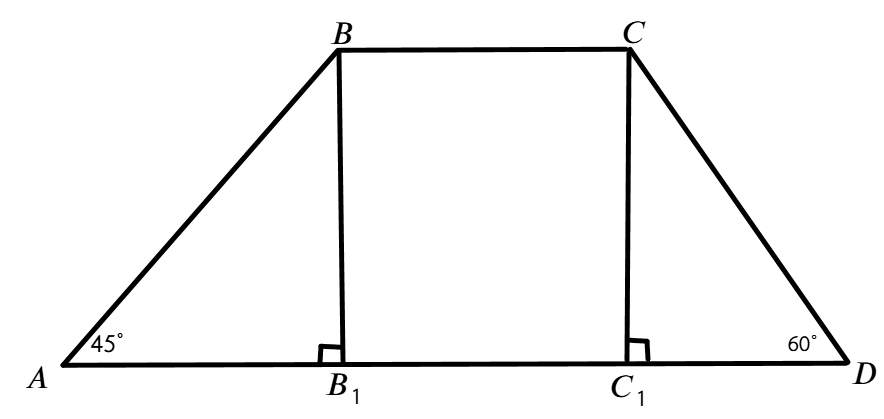
\includegraphics[scale=0.35]{g8-240.png}}
\end{figure}\\
Найдём $AB_1=BB_1 ctg(45^\circ)=6$ и $DC_1=CC_1 ctg(60^\circ)=2\sqrt{3}.$ Так как $BCC_1B_1$ является прямоугольником, $B_1C_1=BC$ и верно соотношение
$S_{ABCD}=\cfrac{1}{2}\cdot6\cdot(BC+BC+6+2\sqrt{3})=42,$ откуда $2BC+6+2\sqrt{3}=14,\ BC=4-\sqrt{3}.$\\
